\documentclass[a5paper,12pt,final]{scrartcl}
%\documentclass[a4paper,12pt,draft]{scrartcl}

\usepackage{url}
\usepackage{ngerman}

% use multiple bibliographies

%\usepackage{multibib}
%\newcites{pap}{References}
%\newcites{app}{ }

% include graphics
\usepackage{graphicx}

% use linenumber
%\usepackage[modulo]{lineno}
%\linenumbers

\usepackage[T1]{fontenc}

% use utf8 encoding
\usepackage[utf8]{inputenc}

% use align environment
\usepackage{amsmath}

% table 3 is multiple pages long
\usepackage{longtable}

% Only for the time of writing
\usepackage{setspace}
\doublespacing

% Citation style in references
\usepackage{natbib}

% Captions auch für nicht-floats
\usepackage{caption}

% for landscape pictures
\usepackage{rotating}

% handle urls
\usepackage{url}

% Title of table of content
\renewcommand\contentsname{Contents}

% Title of bibliography
\renewcommand\refname{References}

% 
\usepackage{ifthen}

%
\usepackage{color}

%% command printing a section titlte page
%% params
%% 1: main title
%% 2: subtitle/author
%% 3: footnote
%% 4: sectionname
%% 5: commands for the last empty page such as  newgeometriy
%% 6: content on backpage
\newcommand{\secpage}[6]
{
	\mbox { }
	\newoddside
	\mbox { }
	% Startseiten-Blatt
	%%% START
	\thispagestyle{empty}
    \helfont
	\mbox{}

	\vfill

	\begin{center}
	{\helfont \Huge  #1}\\[6ex]
	{\fontfamily{phv}\fontsize{18pt}{18pt}\selectfont #2}
	\end{center}
	\vspace{5cm}
	\begin{center}
	\begin{minipage}{0.5\textwidth}
		\begin{center}
		
		\end{center}
	\end{minipage}
	\end{center}
	\vspace{4cm}
	\vfill
	#3
	\addcontentsline{toc}{section}{#4}
	\newpage
	%%% Backpage
    #6
	\mbox { }
	\newoddside
	#5
	\mbox { }
}
%%
%% end newcommand
%%

% provides \isempty
\usepackage{xifthen}
%% new command printing the subsection title and adding this subsectino to the TOC
%% param1: title
%% param2: subsection
%% 3: author
\newcommand{\newsubsec}[3]
{
	\begin{center}
		{\fontfamily{phv}\fontsize{18pt}{18pt}\selectfont #1}
		\ifthenelse{\isempty{#3}}
		{}
		{\\[0.4cm]\fontfamily{phv}\fontsize{14pt}{14pt}\selectfont #3}
	\end{center}
	% add to toc
	\addcontentsline{toc}{subsection}{#2}
}

% slightly large font size
\newcommand{\slarge}{\fontsize{13}{17}\selectfont}

% subsubsection
\newcommand{\newsubsub}[1]
{
    \mbox{ }\newline
    {\noindent \slarge \normalfont \helfont #1}
    \mbox{ }\newline
}


% put the following on an odd page
\newcommand{\newoddside}{
	\ifthenelse{\isodd{\thepage}}{
		\newpage
		\textcolor{white}{placeholder} 
		%\thispagestyle{empty}
		\newpage
	}
	{\newpage}

}

% space between two letters
\newcommand{\newletter}{
	\vspace{1.5cm}
}

% page margins
\usepackage{geometry}
\geometry{a4paper,bottom=3cm, top=2.5cm, left=2.8cm, right=2.3cm}

% we do not want to have section numbers (but a TOC).
\setcounter{secnumdepth}{-1}

% use linux libertine as font
\usepackage[T1]{fontenc}
%\usepackage{libertine}
%\renewcommand*\oldstylenums[1]{{\fontfamily{fxlj}\selectfont #1}}

% http://www-h.eng.cam.ac.uk/help/tpl/textprocessing/fonts.html
%% Enable helvetica font
\usepackage{helvet}
%\usepackage{avant} \renewcommand{\familydefault}{\sfdefault}
%\usepackage{newcent} \renewcommand{\familydefault}{\sfdefault}
%\usepackage{bookman} \renewcommand{\familydefault}{\sfdefault}

%% Control the fonts and formatting used in the table of contents.
\usepackage{tocloft}
%\renewcommand{\cftsecaftersnumb}{\rlap{\rule[-2.5mm]{0.5\textwidth}{.4pt}}}
%\renewcommand{\cftsecaftersnum}{\hspace{4mm}\rule[-2.5mm]{0.5\textwidth}{.4pt}\hss}

% TOC title
\renewcommand{\cfttoctitlefont}{\Large\normalfont\bfseries}
% section
\renewcommand{\cftsecfont}{\large\normalfont\bfseries}
% section page number
\renewcommand{\cftsecpagefont}{\normalfont}


% activate helvetica as default font
\newcommand{\helfont}{
    %\renewcommand{\familydefault}{\sfdefault}
    \fontfamily{phv}\selectfont
}

% standard latex font?
\newcommand{\oldfont}{
%    \renewcommand{\familydefault}{\rmdefault}
    \fontfamily{\rmdefault}\selectfont
}


%%
%% Redefine section headings
%%
\makeatletter
\renewcommand\section{\@startsection{section}{1}{\z@}%
                     {-3.5ex \@plus -1ex \@minus -.2ex}%
                     {2.3ex \@plus.2ex}%
                     {\normalfont\Large\bfseries}}


\makeatother

%% background picture for first page
\usepackage{tikz}
\usepackage{eso-pic}
\newcommand\BackgroundPic{
    \put(-10,0){
        \parbox[b][\paperheight]{\paperwidth}{%
        \vfill
        \centering
        
\begin{tikzpicture}%
            \node[opacity=0.15]{%was: 0.6
                 % width=0.85 for all except variant 3
                \includegraphics[height=\paperheight,
                keepaspectratio]{bg.jpg}%
            };
%                \includegraphics[width=\paperwidth,height=\paperheight,
        \end{tikzpicture}
%        \vspace{5cm}
        \vfill
}}}

\newcommand\BackgroundPicTitle{
    \put(-10,0){
        \parbox[b][\paperheight]{\paperwidth}{%
        \vfill
        \centering
        
\begin{tikzpicture}%
            \node[opacity=0.55]{%was: 0.6
                 % width=0.85 for all except variant 3
                \includegraphics[height=\paperheight,
                keepaspectratio]{bg.jpg}%
            };
%                \includegraphics[width=\paperwidth,height=\paperheight,
        \end{tikzpicture}
%        \vspace{5cm}
        \vfill
}}}
\begin{document}
\AddToShipoutPicture*{\BackgroundPicTitle}
\helfont
%\fontsize{15pt}{15pt}\selectfont
%\fontsize{14pt}{14pt}\selectfont
%\fontsize{14pt}{13pt}\selectfont
%\fontsize{12pt}{12pt}\selectfont

\thispagestyle{empty}
\mbox{}

\vfill

\begin{center}
{\oldfont\fontsize{34pt}{34pt}\selectfont \textbf{Vegetarische Gerichte}}\\[6ex]

\end{center}
\vspace{3cm}
\vfill
\begin{center}
    \textbf{https://github.com/m-weigand/VegetarischeKochrezepte}
\end{center}
\vfill
\begin{center}
    \textbf{Lizenz: Attribution-ShareAlike 4.0 International (CC BY-SA 4.0)}\\
    https://creativecommons.org/licenses/by-sa/4.0/
\end{center}

\newpage
\thispagestyle{empty}
\AddToShipoutPicture{\BackgroundPic}
\begin{center}
    {Zusammengestellt von Maximilian Weigand (mweigand@mweigand.net), September 2016, Ausgabe 5}
\end{center}
\vfill
\begin{center}

\end{center}
\newpage
\thispagestyle{empty}
\mbox{ }
\vspace{-1cm}
\renewcommand*\contentsname{Inhaltsverzeichnis}
\setcounter{tocdepth}{2}
\tableofcontents
%%% Seite 4
\newpage
%\thispagestyle{empty}
\mbox{ }
%\vfill
%\mbox{}\hfill  \hfill \mbox{ }
\newpage
\mbox{}\hfill  \hfill \mbox{ }
\newpage

\section{Bauern Omlette}
% Linke Seite: Rezept
Zutaten:
\begin{itemize}
    \item 1 rote Paprika
    \item 1 rote Zwiebel
    \item 400g Kartoffeln
    \item 5 Eier
    \item 2 El Milch
    \item Salz und Pfeffer
    \item 1 Tl getrockneten Thymian
    \item Paprikapulver
	\item 1/2 Päckchen gefriergetrocknete Kräuter aus dem gutsortierten
		Tiefkühlsortiment
    \item Aiwar
\end{itemize}

\noindent Zubereitung:

\noindent Kartoffeln fest kochen. Zwiebeln und Paprika klein schneiden und an
Öl anschwitzen. Kartoffeln dazu schneiden und vermischen. Auf mittlerer Hitze
braten lassen und regelmäßig umrühren. Eier aufschlagen und mit Milch
verrühren, Salz, Pfeffer, Paprikapulver und die Kräuter unterrühren. Wenn die
Kartoffeln schön knusprig sind, das Rührei dazugeben und ordentlich vermischen.
Sobald das Omlette goldig-braun ist, mit Aiwar servieren.

% Recht Seite: Bild
\newpage
\mbox{}
\vfill
\begin{center}
    % 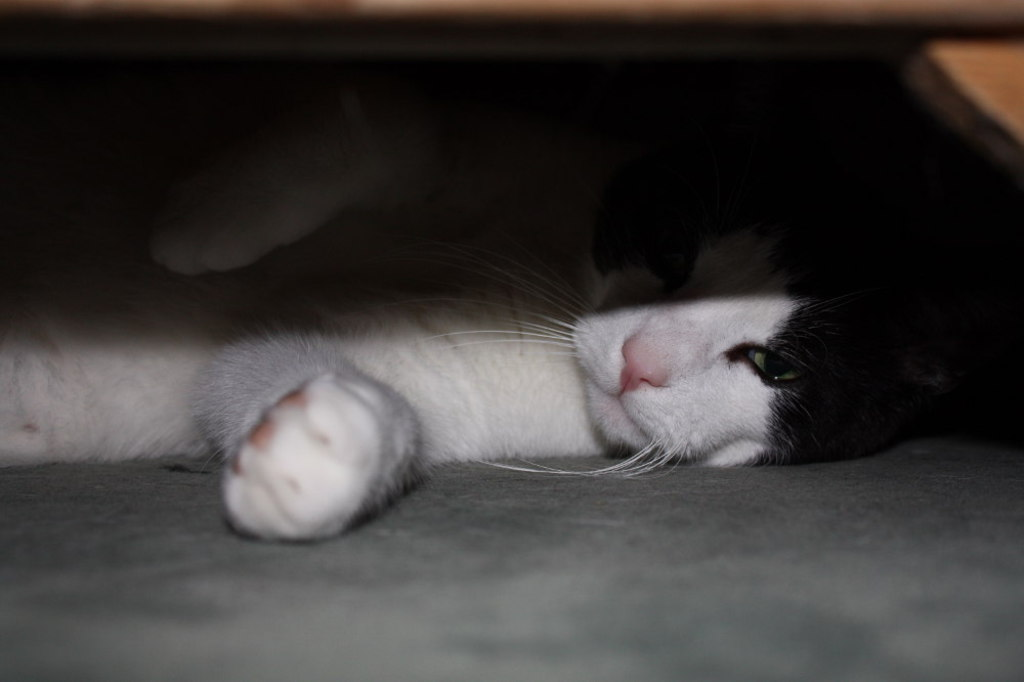
\includegraphics[width=\textwidth]{Bauern-Omlette/filler.jpg}
\end{center}
\vfill
\mbox{ }
\newpage

\section{Kubanisches Reisgericht}
% Linke Seite: Rezept
Zutaten (4 Personen):
\begin{itemize}
    \item 3 Bananen
    \item 1 Zwiebel
    \item 1 grüne Paprika
    \item 1 Dose Tomaten
    \item 1-2 Knoblauchzehen
    \item 1 Dose Kidneybohnen
    \item Salz und Pfeffer
    \item 250g Reis
\end{itemize}

\noindent Zubereitung:

\noindent Zwiebeln, Knoblauch und Paprika klein schneiden und etwas Öl
anschwitzen. Tomaten,Reis und etwa 450 ml Wasser dazugeben und mit Salz und
Pfeffer würzen. Umrühren und aufkochen lassen und bei schwacher Hitze etwa 25
Minuten köcheln lassen, bis der Reis gar ist. Bei Bedarf mit Paprika-Pulver
oder Mexiko-Pulver würzen (ist aber nicht nötig).

\noindent Bananen halbieren und in einer Pfanne bei mittlerer Hitze anbraten,
bis sie leicht karamellisiert sind. Zum Reis servieren.

% Recht Seite: Bild
\newpage
\mbox{}
\vfill
\begin{center}
    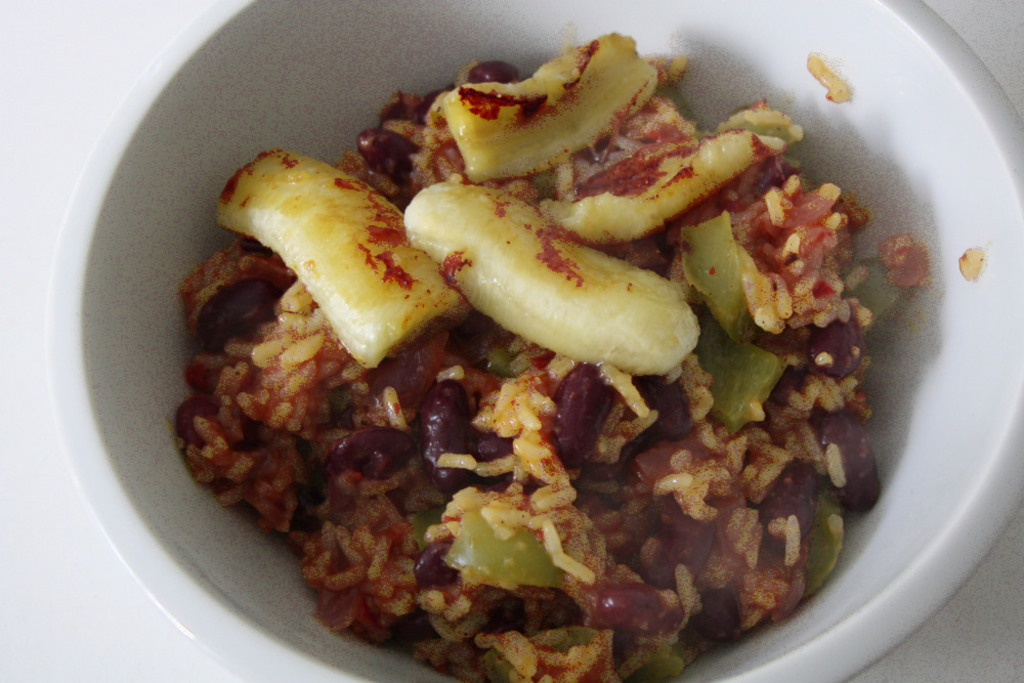
\includegraphics[width=\textwidth]{Kubanisches-Reisgericht/IMG_3600._small.jpg}
\end{center}
\vfill
\mbox{ }
\newpage

\section{Cashew Ringelnudeln}
% Linke Seite: Rezept
Zutaten:
\begin{itemize}
    \item Ringelnudeln
    \item Asia-Gemüse (tiefgekühlt)
    \item Ketjap Manis (1 EL)
    \item Cashew Nüsse
\end{itemize}

\noindent Zubereitung:

\noindent Cashew Nüsse in einer Pfanne bei mittlerer Hitze anrösten, bis
sie schön braun sind. Gleichzeitig Ringelnudeln in separatem Topf kochen
(leicht salzen). Cashews aus der Pfanne nehmen und Gemüse an Ketjap Manis
auftauen und kurz köcheln lassen. Dann Nudeln und Cashews dazugeben und
verrühren. Mit Salz und Pfeffer abschmecken.

% Recht Seite: Bild
\newpage
\mbox{}
\vfill
% \begin{center}
%     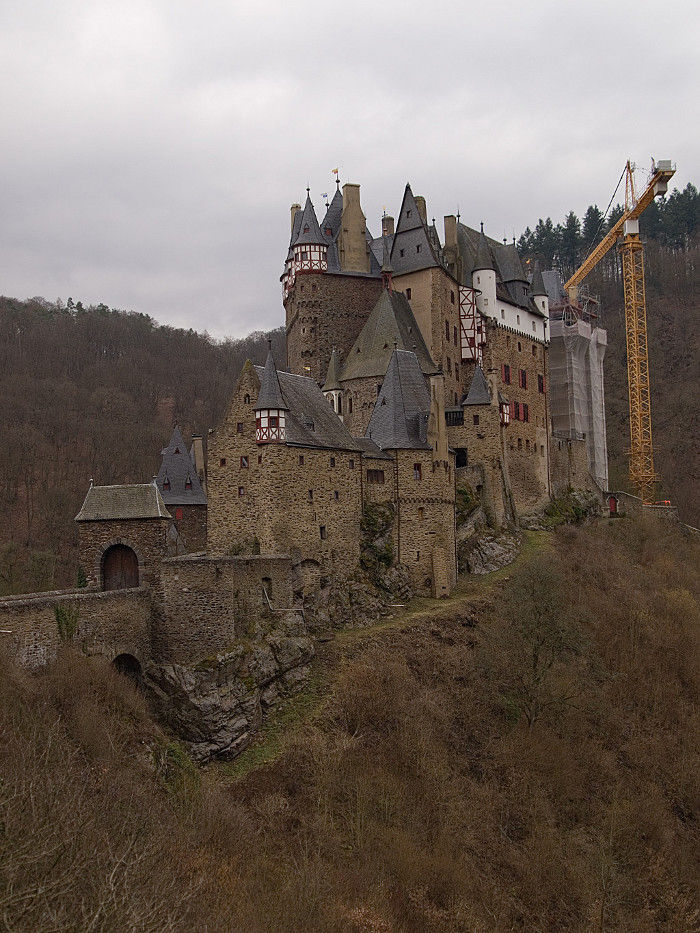
\includegraphics[width=0.8\textwidth]{Cashew-Ringelnudeln/burg.jpg}
% \end{center}
\vfill
\mbox{ }
\newpage

\section{Couscous Auflauf}
% Linke Seite: Rezept
Zutaten:
\begin{itemize}
    \item 1 El Olivenlk
    \item 1 große Zwiebel
    \item 1 Knoblauchzehe
    \item 1-2 Fenchelknollen
    \item 1 El Balsamico-Essig
    \item 250g rote (oder gelbe) Linsen
    \item 1 Dose geschälte Tomaten (ca. 300g)
    \item 40g Tomatenmark
    \item 1 Tl getrockneten Thymian
    \item 200g Couscous
    \item 200g Hüttenkäse
    \item 80g Feta
\end{itemize}

\noindent Zubereitung:

\noindent Linsen in kleinem Topf mit reichlich Gemüsebrühe aufkochen und ziehen lassen, bis sie leicht sähmig sind.

Öl in einem Topf erhitzen, Zwiebel und Knoblauch schälen, fein hacken, und etwas 3 Minuten darin andünsten. Fenchel putzen, in Streifen schneiden und dazugeben. Alles etwa 3 min dünsten. Mit Essig ablöschen und 100ml Wasser dazu geben. Köcheln lassen bis der Fenchel weich ist. Linsen und Tomaten dazu geben, Tomatenmark und Thymian unterrühren und alles noch mal aufkochen lassen. Mit Salz und Pfeffer abschmecken.

Couscous in geölte Auflaufform geben, eine Prise Salz dazu, und mit kochendem Wasser übergießen, so dass der Couscous etwa 1 cm hoch bedeckt ist. Couscous ausquellen lassen.

Das gekochte Gemüse auf dem gequollenen Couscous verteilen, mit Hüttenkäse und Feta bedecken.

Im Backofen bei $200^\circ$ 30-40 Minuten goldgeben überbacken.
%% Recht Seite: Bild
%\newpage
\mbox{}
\vfill
\begin{center}
    \includegraphics[width=\textwidth]{Couscous-Auflauf/IMG_6094.JPG}
\end{center}
\vfill
\mbox{ }
\newpage

\section{Gnocchi in Tomatensauce}
% Linke Seite: Rezept
Zutaten:
\begin{itemize}
    \item Tomatensauße mit Kräutern (von DM)
    \item Gnocchi
    \item 1 El Öl
    \item Salz und Pfefffer
    \item getrockneter Thymian
\end{itemize}

\noindent Zubereitung:

\noindent Gnocchi in Pfanne mit ordentlich Öl gelb-braun braten. Tomatensauße dazu geben und mit Salz, Pfeffer, und Thymian abschmecken.

% Recht Seite: Bild
\newpage
\mbox{}
\vfill
\begin{center}
%    \includegraphics[width=\textwidth]{}
\end{center}
\vfill
\mbox{ }
\newpage

\section{Hummus}
% Linke Seite: Rezept
Zutaten:
\begin{itemize}
    \item 1 Dose gekochten Kichererbsen (ca. 800g)
    \item 1-2 El. Tahina (Sesam-Mus)
    \item Salz und Pfeffer
    \item 1/2 Zitrone
    \item (Beilage) Tortillas
    \item (Beilage) Jasmin-Reis
\end{itemize}


\noindent Zubereitung:

\noindent Kichererbsen in Topf füllen und leicht mit Wasser becken. Zugedeckt etwa 20 Minuten kochen. Wasser abschütten und 2 El. Wasser hinzugeben. Zitronensaft der 1/2 Zitrone zugeben. Tahina hinzugeben. Alles pürieren. Mit Salt, Pfeffer, und zusätzlichem Tahina abschmecken.

Mit Reis in Tortillas einrollen und servieren.

% Recht Seite: Bild
\newpage
\mbox{}
\vfill
\begin{center}
    \includegraphics[width=\textwidth]{Hummus/IMG_6096.JPG}
\end{center}
\vfill
\mbox{ }
\newpage

\section{Ingwer-Curry}
% Linke Seite: Rezept
Zutaten:
\begin{itemize}
    \item
\end{itemize}

Zubereitung:

% Recht Seite: Bild
\newpage
\mbox{}
\vfill
\begin{center}
%    \includegraphics[width=\textwidth]{}
\end{center}
\vfill
\mbox{ }
\newpage

\section{Ingwer-Zwiebel-Gericht}
% Linke Seite: Rezept
Zutaten (ca. 6 Portionen):
\begin{itemize}
    \item 2 rote Zwiebeln
	\item Frühlingszwiebeln
    \item 1 Knoblauchzehe
    \item 3 cm Ingwer-Knolle
    \item Salz und Pfeffer
	\item 1-2 Löffel Curry
	\item 0.5 Koreanderpulver
	\item Paprika
	\item kleine Tomaten
	\item (vielleicht) Porre
	\item geröstere Erdnusse
	\item Ketjap Manis
    \item (Beilage) Reisnudeln
\end{itemize}

\noindent Zubereitung:



\noindent % Recht Seite: Bild
\newpage
\mbox{}
\vfill
\begin{center}
    % 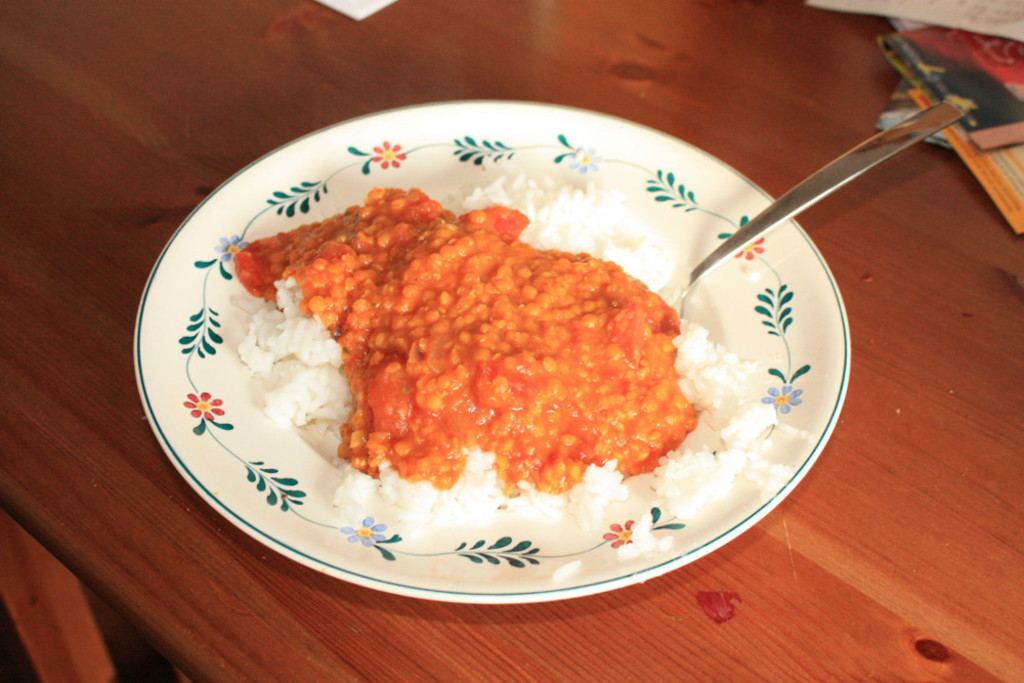
\includegraphics[width=\textwidth]{Ingwer-Curry/IMG_6088._small.jpg}
\end{center}
\vfill
\mbox{ }
\newpage

\section{Kartoffelecken}

\textbf{Gelingt schnell und einfach}

% Linke Seite: Rezept
Zutaten:
\begin{itemize}
    \item 1 kg Kartoffeln
    \item Olivenöl
    \item getrockneter Thymian
    \item Salz und Pfeffer
\end{itemize}

\noindent Zubereitung:

\noindent Ofen auf etwa 230 Grad vorwärmen. Kartoffeln waschen und in kleine Würfel von etwa 1 cm Kantenlänge schneiden. Danach in einer Schüssel Öl, Thymian, Salz, und Pfeffer, und Kartoffeln vermischen. Kartoffeln auf einem Blech ausbreiten und etwa 30 Minunten im Ofen garen und rösten lassen. Lecker!

% Recht Seite: Bild
\newpage
\mbox{}
\vfill
\begin{center}
%    \includegraphics[width=\textwidth]{}
\end{center}
\vfill
\mbox{ }
\newpage

%TODO\section{Kartoffel-gratin}
% Linke Seite: Rezept
Zutaten:
\begin{itemize}
    \item
\end{itemize}

Zubereitung:

% Recht Seite: Bild
\newpage
\mbox{}
\vfill
\begin{center}
%    \includegraphics[width=\textwidth]{}
\end{center}
\vfill
\mbox{ }
\newpage

%TODO\section{Käsepfannkuchen}
% Linke Seite: Rezept
Zutaten:
\begin{itemize}
    \item
\end{itemize}

Zubereitung:

% Recht Seite: Bild
\newpage
\mbox{}
\vfill
\begin{center}
%    \includegraphics[width=\textwidth]{}
\end{center}
\vfill
\mbox{ }
\newpage

\section{Kubanisches Reisgericht}
% Linke Seite: Rezept
Zutaten (4 Personen):
\begin{itemize}
    \item 3 Bananen
    \item 1 Zwiebel
    \item 1 grüne Paprika
    \item 1 Dose Tomaten
    \item 1-2 Knoblauchzehen
    \item 1 Dose Kidneybohnen
    \item Salz und Pfeffer
    \item 250g Reis
\end{itemize}

\noindent Zubereitung:

\noindent Zwiebeln, Knoblauch und Paprika klein schneiden und etwas Öl
anschwitzen. Tomaten,Reis und etwa 450 ml Wasser dazugeben und mit Salz und
Pfeffer würzen. Umrühren und aufkochen lassen und bei schwacher Hitze etwa 25
Minuten köcheln lassen, bis der Reis gar ist. Bei Bedarf mit Paprika-Pulver
oder Mexiko-Pulver würzen (ist aber nicht nötig).

\noindent Bananen halbieren und in einer Pfanne bei mittlerer Hitze anbraten,
bis sie leicht karamellisiert sind. Zum Reis servieren.

% Recht Seite: Bild
\newpage
\mbox{}
\vfill
\begin{center}
    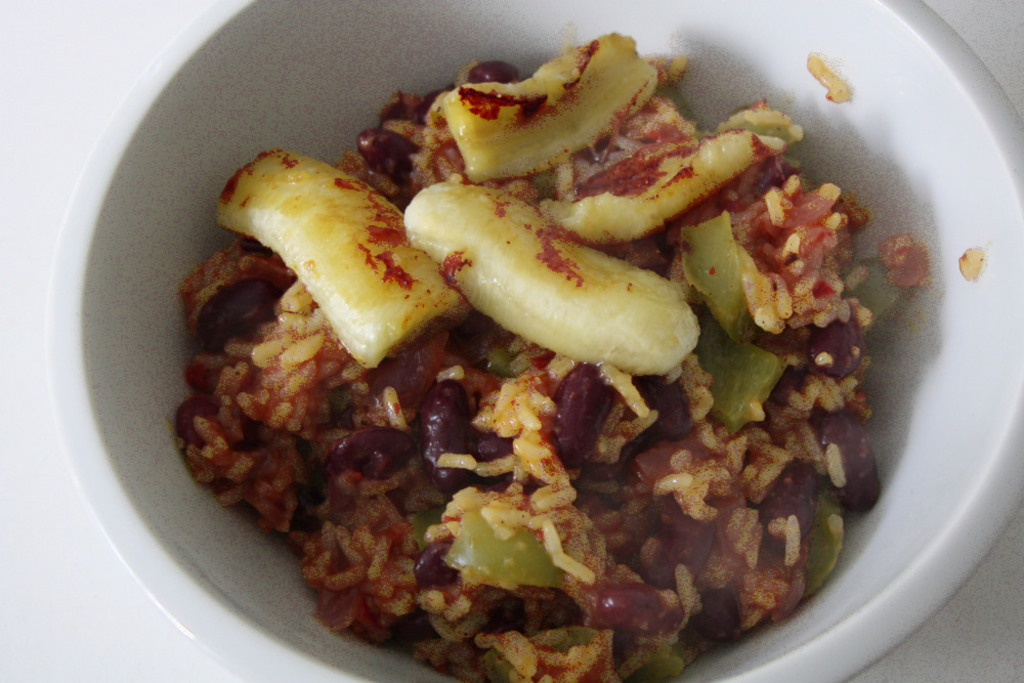
\includegraphics[width=\textwidth]{Kubanisches-Reisgericht/IMG_3600._small.jpg}
\end{center}
\vfill
\mbox{ }
\newpage

\section{Kichererbsen Curry}
% Linke Seite: Rezept
Zutaten:
\begin{itemize}
    \item 1 Dose Kichererbsen (vorgekocht)
    \item 2 Paprika (rot und gelb)
    \item 1-2 Fenchel
    \item Zucchini (Wenn vorhanden)
    \item 1 Dose Kokusnusmilch
    \item 1 Dose Tomaten (oder entsprechende Menge frische Tomaten)
    \item 1 Strauch Frühlingszwiebeln
    \item (optional) 1 Dose Cashew-Nüsse
    \item 1 Glas rote Currypaste
\end{itemize}

\vspace{1cm}

\noindent Zubereitung:

\noindent Gemüse kleinschneiden. Kichererbsen abtropfen. Die Hälfte der
Currypaste in einer Pfanne (oder Wok) kurz anbraten, dann Gemüse hinzugeben und
zugedeckt bei mittlerer Hitze dünsten lassen. Nach etwa 10 Minuten Kichererbsen
dazu geben. Wenn das Gemüse den gewünschten Härtegrad hat, Kokusmilch
hinzugeben und aufkochen lassen. Mit Pfeffer und Salz abschmecken und mit Reis
servieren.

% Recht Seite: Bild
\newpage
\mbox{}
\vfill
\begin{center}
    \includegraphics[width=0.5\textwidth]{Kichererbsen-Curry/IMG_6111.JPG}
\end{center}
\vfill
\begin{center}
    \includegraphics[width=\textwidth]{Kichererbsen-Curry/IMG_6085.JPG}
\end{center}
\vfill
\mbox{ }
\newpage

\section{Kürbissuppe}
% Linke Seite: Rezept
Zutaten:
\begin{itemize}
    \item 2 Zwiebeln
    \item kleiner Hokaidokürbis (mit zwei Händen umfassbar sein)
    \item 2-6 Möhren (nach Geschmack)
    \item (optional) 1 Süßkartoffel
    \item 1 Stück Ingwer (\~ 2 cm)
    \item Salz, Pfeffer, Chilli
    \item 1 Knoblauchzehe
    \item 2 Löffel Gemüsebrühe
    \item Kürbiskerne
    \item Baguette
\end{itemize}

\noindent Zubereitung:

Möhren kleinschneiden; Kürbis teilen, Kerne rausholen, und dann kleinschneiden
(etwa 2x2x2 $cm^2$). Süßkartoffel schälen und ebenfalls kleinschneiden.

Zwiebeln kleinschneiden, mit Knoblauch (und einer kleinen Chilli) anbraten,
danach Mühren, Kürbis, und Süßkartoffeln dazu geben. Wasser dazugeben, bis alle
knapp unter Wasser steht. Gemüsebrühe dazugeben, gut rühren. Solange kochen,
bis alles weich ist (mit Gabel testen). Ingwer reinreiben. Salz/Pfeffer
dazugeben und alles pürieren. Eventuell noch etwas Wasser verkochen lassen, bis
die Suppe die gewünschte Dicke hat.

Kürbiskerne in einer Pfanne anrösten und zusammen mit Baguette zur Suppe
servieren.
\noindent
% Recht Seite: Bild
%\newpage
\mbox{}
\vfill
\begin{center}
%    \includegraphics[width=\textwidth]{}
\end{center}
\vfill
\mbox{ }
\newpage

\section{Korma-Curry}
% Linke Seite: Rezept
Zutaten:
\begin{itemize}
    \item
\end{itemize}

Zubereitung:

% Recht Seite: Bild
\newpage
\mbox{}
\vfill
\begin{center}
%    \includegraphics[width=\textwidth]{}
\end{center}
\vfill
\mbox{ }
\newpage

\section{Maronen}
% Linke Seite: Rezept
Zutaten:
\begin{itemize}
    \item Maronen (vorgekocht, in Dose oder verschweißt)
    \item Butter
    \item Zucker
    \item 2 Löffel Gemüsebrühe
\end{itemize}

\noindent Zubereitung:

Butter und Zucker anbraten, bis beides flüssig geworden ist. Umrühren, und mit
ein bischen Gemüsebrühe abschrecken. Maronen dazugeben ud gut umrühren. Kurz
anköcheln lassen, und dann karamelisieren lassen.

\noindent
% Recht Seite: Bild
%\newpage
\mbox{}
\vfill
\begin{center}
%    \includegraphics[width=\textwidth]{}
\end{center}
\vfill
\mbox{ }
\newpage

\section{Möhren-Kohl Curry}
% Linke Seite: Rezept
Zutaten:
\begin{itemize}
    \item 1 Packung Möhren
    \item 1 Chinakohl
    \item Curry-Pulver
    \item Salz und Pfeffer
    \item Öl
    \item 2 Gläser rote oder gelbe Linsen
    \item Gemüsebrühe
    \item (Beilage) Jasmin-Reis
\end{itemize}

\noindent Zubereitung:

\noindent Linsen mit Wasser (1:2) und Gemüsebrühe in einem kleinen Topf
aufkochen und ziehen lassen.

Möhren und Kohl in kleine Stücke schneiden. Möhren mit zusammen mit etwa 1 El
Öl und 1-2 El Curry-Pulver scharf anbraten. Dann Kohl hinzugeben und
vermischen. Bei mittlerer Hitze zugedeckt 10-20 Minuten köcheln lassen, bis die
Möhren gar sind. Sähmige Linsen dazugeben und nach Wunsch etwa einköcheln
lassen. Mit Salz, Pfeffer, und Curry-Pulver abschmecken. Mit Reis servieren.

% Recht Seite: Bild
\newpage
\mbox{}
\vfill
\begin{center}
%    \includegraphics[width=\textwidth]{}
\end{center}
\vfill
\mbox{ }
\newpage

\section{Pfannkuchen}

% Linke Seite: Rezept
Zutaten:

\begin{itemize}
    \item 4 Eier
	\item 400g Mehl
	\item 100ml Sprudelwasser
	\item 400ml Milch
	\item 1 Packung Vanillezucker
	\item Salz/Pfeffer
\end{itemize}

\noindent Zubereitung:

\noindent


% Recht Seite: Bild
\newpage
\mbox{}
\vfill
\begin{center}
    % \includegraphics[width=\textwidth]{}
\end{center}
\vfill
\mbox{ }
\newpage

\section{Rote-Linsen Suppe}
% Linke Seite: Rezept
Zutaten:
\begin{itemize}
	\item Zutaten (für 2-4 Portionen):
	\item 1 Packung passierte Tomaten (500 g)
	\item 1 Dose Kokosmilch(400 g)
	\item 1-2 Zwiebel(n)
	\item 300 g	Linsen, rote
	\item 3 TL	Chilipulver
	\item 2 TL	Kurkuma
	\item 300 ml Gemüsebrühe + (ca. 50-100 ml zum Ausspülen der Tomatenpackung)
	\item Sonnenblumenöl
	\item Salz
	\item Zusatz Maxi: Eine Tasse Bulgur
\end{itemize}

\url{http://www.chefkoch.de/rezepte/1718481280523737/Rote-Linsen-Kokos-Suppe.html}

\noindent Zubereitung:

\begin{itemize}
	\item Rote Linsen gut waschen.
	\item Zwiebeln klein schneiden und mit etwas Öl, Currypulver, und Chillis
		anschwitzen.
	\item Rote Linsen, Tomaten, Kokosmilch, und Gemüsebrühe zugeben.
	\item 10-20 Minuten köcheln lassen, mit Gewürzen abschmecken.
	\item Nach Möglichkeit ziehen lassen.
\end{itemize}

\noindent
% Recht Seite: Bild
%\newpage
\mbox{}
\vfill
\begin{center}
%    \includegraphics[width=\textwidth]{}
\end{center}
\vfill
\mbox{ }
\newpage

\section{Salatsauße}

% Linke Seite: Rezept
Zutaten:

\begin{itemize}
    \item 2 Löffel Balsamicoessig
	\item 1 Löffel Distelöl
	\item 1 Löffel Olivenöl
	\item 1 kleiner Löffel Salz
	\item 1 kleiner Löffel Pfeffer
	\item 1 kleiner Löffel Zucker
	\item 1 kleiner Löffel Kräuter Provincial
\end{itemize}

\noindent Zubereitung:

\noindent


% Recht Seite: Bild
\newpage
\mbox{}
\vfill
\begin{center}
    % \includegraphics[width=\textwidth]{}
\end{center}
\vfill
\mbox{ }
\newpage

\section{Schupfnudeln mit Satee-Sauce}

\textbf{Schnell, gelingt immer}

% Linke Seite: Rezept
Zutaten:
\begin{itemize}
    \item 1 Packung Schupfnudeln
    \item 1 El Rapsöl
    \item 1 Packung Sate-Sauce
\end{itemize}

\noindent Zubereitung:

\noindent Schupfnudeln gold-braun braten im Öl. Sate-Sauce unterrühren. Lecker!

% Recht Seite: Bild
\newpage
\mbox{}
\vfill
\begin{center}
    \includegraphics[width=0.5\textwidth]{Schupfnudeln-Satee/IMG_6114.JPG}
    \vfill
    \includegraphics[width=\textwidth]{Schupfnudeln-Satee/IMG_6108.JPG}
\end{center}
\vfill
\mbox{ }
\newpage

\section{Sherry Risotto}
% Linke Seite: Rezept
Zutaten:
\begin{itemize}
    \item 1 Flasche Sherry
    \item 1 Packung Risotto-Reis
    \item 1 Packung (~5) Spitzpaprika, oder 3 rote Paprika
    \item 1 rote Zwiebel
    \item Mexiko-Gewürzsalz/-Pulver
    \item Salz und Pfeffer
    \item Cashew-Nüsse
    \item 
\end{itemize}

\noindent Zubereitung (im großen Wok):

\noindent Cashews bei mittlerer Hitze rösten. In einer Schüssel zwischenlagern.

Zwiebeln in Öl anschwitzen, Reis dazu und kurz anbraten lassen. Dann mit
Sherry ablöschen und kleingeschnittene Paprika dazu. Halbe Flasche
Risotto dazu. Cashews wieder hinzugeben. Etwa 30-40 Minuten bei niedriger Hitze köcheln lassen. Bei
Bedarf Wasser oder Sherry nachfüllen. Regelmäßig umrühren, damit nichts
am Boden anbrennt. Nach etwa 20 Minuten Gewürze hinzugeben. Etwa 2 El
Mexiko-Pulver, Salz, und Pfeffer. Das ganze solange köcheln lassen, bis
der Reis gut gequollen ist. Danach mit den Gewürzen noch einmal abschmecken. Am besten danach bei abgeschaltetem Herd noch 30 Minuten warten, damit der Reis richtig gut durchzieht.

% Recht Seite: Bild
\newpage
\mbox{}
\vfill
\begin{center}
%    \includegraphics[width=\textwidth]{}
\end{center}
\vfill
\mbox{ }
\newpage

\section{Schokocreme}

% Linke Seite: Rezept
Zutaten:

\begin{itemize}
    \item 3 Eier
	\item 150g helle/dunkle Schokolade (Konfitüre)
	\item 0.5 Liter Sahne
	\item 1 Packung Mohnfix
	\item Portion Contreau
\end{itemize}

\noindent Zubereitung:

\noindent 3 frische Eier schaumig schlagen. 150g dunkle/\textbf{helle}
Schokolade/Kuvertüre in der Mikrowelle warmmachen (mehrmals umrühren,
Schokolade brennt schnell an). Warme Schokolade langsam mit Schneebesen unter
die schaumigen Eier unterheben. Mohnfix unterheben. Contreau zugeben.

\noindent Für einige Stunden kaltstellen.

\noindent Sahne steifschlagen und unterheben (eventuell etwas weniger Sahne
nehmen).

\noindent Für dunkle Schokolade kein Mohnfix nehmen.


% Recht Seite: Bild
\newpage
\mbox{}
\vfill
\begin{center}
    % \includegraphics[width=\textwidth]{}
\end{center}
\vfill
\mbox{ }
\newpage

\section{Vegetarisches Chilli}
% Linke Seite: Rezept
Zutaten:
\begin{itemize}
    \item 2 Dosen Kidneybohnen
    \item ca. 200ml Bulgur
    \item 3 Dosen (ca. 600g) geschälte und gehackte Tomaten
    \item 2 Knoblauchzehen
    \item je 1 Tasse (gehackt/klein geschnitten):
        \begin{itemize}
            \item Zwiebeln
            \item Sellerie (oder Lauch)
            \item Möhren
            \item Paprika
        \end{itemize}
    \item 1/2 Zitrone
    \item 1 Tl gemahlener Kümmel
    \item 1 Tl Basilikum
    \item 1 Tl Chilli
    \item Salz und Pfeffer
    \item 3 El Tomatenmark
    \item 3 El trockener Rotwein
    \item Olivenöl
    \item (Beilage) 1 frisches Baguette
\end{itemize}

Zubereitung:
In einem großen Topf die Zwiebeln und das Chilli andünsten. Das restliche Gemüse (außer den Tomaten) dazugeben. Alle vermischen und Salzen und Pfeffern. Dann bei geringer Hitze ca. 15 Minuten dünsten, bis das Gemüse gar ist (die Möhren testen!).

In einem zweiten Topf die Tomaten aufkochen und den Bulgur dazugeben. Ca. 20 Minuten ziehen lassen. Wenn der Bulgur danach noch nicht weich  ist, nochmal etwas Wasser dazugeben und erneut aufkochen lassen.

Gemüse mit Rotwein ablöschen und Zitronensaft dazugeben. Tomatenmark und die restlichen Gewürze untermischen.

Die Kidneybohnen und den Bulgur dazugeben. Alles vermischen und nochmal kurz aufkochen. Mit Salz und Pfeffer abschmecken.

Mit frischem Baguette servieren.

% Recht Seite: Bild
\newpage
\mbox{}
\vfill
\begin{center}
%    \includegraphics[width=\textwidth]{}
\end{center}
\vfill
\mbox{ }
\newpage

\section{Zucchini Curry}
% Linke Seite: Rezept
Zutaten:
\begin{itemize}
    \item 1 Kg Zucchini
    \item 1 gelbe Paprika
    \item 200g gelbe (oder rote) Linsen
    \item Gemüsebrühe
    \item Currypuler
    \item Salz und Pfeffer
    \item getrockneten Thymian
    \item Olivenöl
    \item (Beilage) Jasmin-Reis
\end{itemize}

\noindent Zubereitung:

\noindent Zucchini in Stücke schneiden und Paprika klein würfeln. Ca. 2 Tl
Currypulver im Öl anschwitzen, danach Zucchini, Paprika und Thymian dazugeben.
Gar dünsten.

Gleichzeitig in 400 ml Gemüsebrühe aufkochen, dann ca. 10 Minuten ziehen
lassen, bis sie weich sind, sonst noch mal aufkochen lassen.

Linsen und Zucchinigemüse vermischen. Mit Salt und Pfeffer abschmecken.

Mit Reis servieren.
% Recht Seite: Bild
\newpage
\mbox{}
\vfill
\begin{center}
    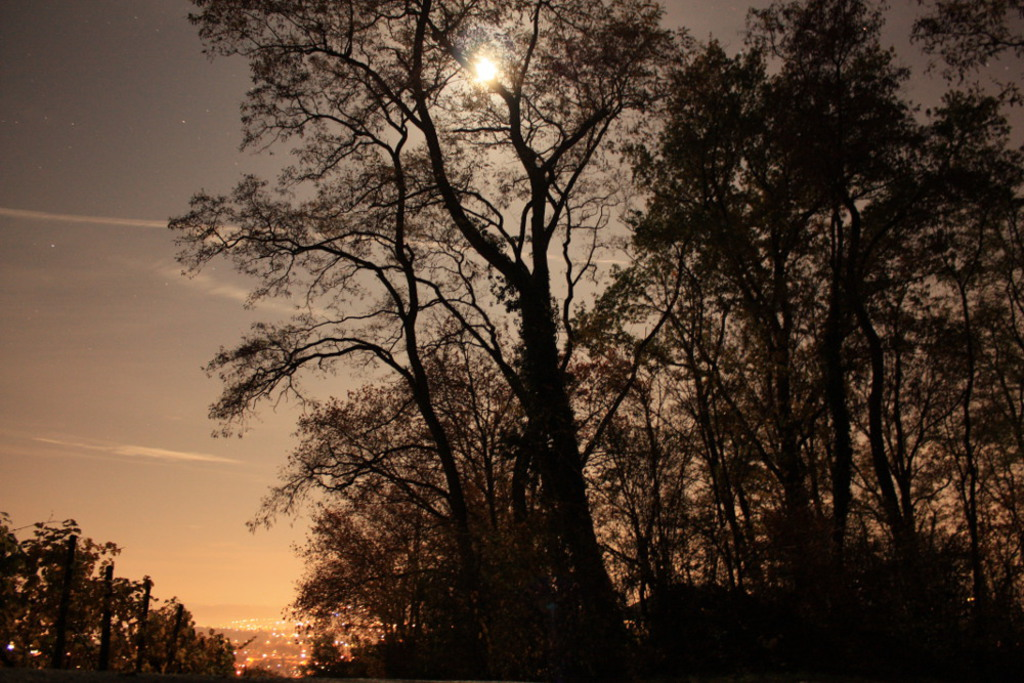
\includegraphics[width=\textwidth]{Zucchini-Curry/IMG_5831_small.jpg}
\end{center}
\vfill
\mbox{ }
\newpage

\section{Diverses}

\textbf{Auberginen}

In Scheiben schneiden, mit Salz Wasser austreiben, dann in
viel Fett anbraten. So verlieren die Auberginen ihre Zähigkeit.

\vspace{2cm}

\textbf{Couscousgericht (Experimentell)}

\begin{itemize}
    \item Zwiebeln/Knoblauch/Chillies/Tofu in Fett anbraten
    \item Frühlingszwiebeln/Fenchel gut anbraten
    \item Paprika/Tomaten/Zitrone dazugeben
    \item etwa 1 Tasse Wasser mit Gemüsebrühe dazu
    \item 200g Couscous dazu, Hard runterdrehen lassen und köcheln lassen
    \item Minze dazu
    \item Tomatenmark/Kreuzkümmel dazu
\end{itemize}


\newpage


\end{document}

